\chapter{Trust in Cameroon}
\begin{abstract}
Two common features of fragile states are a lack of market access, and a lack of social capital. In this paper, we explore the behavioural links between these two features. Using the results from an Investment Game played with over 3,000 rural household in Northern Cameroon, we examine how the determinants of trusting behaviour change across a market integration gradient. We find that expectations about reciprocal behaviour, a commonly used definition of trust, do not drive trusting behaviour in non-market communities, but it does in market communities. We argue that this is not due to any difference in expectations, but due to a learning effect, where the increased exposure to interactions with strangers afforded by markets has a positive effect on the willingness to engage in trusting behaviour.
\end{abstract}


%%%%%%%%%%%%%%%%%%%%%%%%%%
\section{Introduction}
%%%%%%%%%%%%%%%%%%%%%%%%%%
%hook

%line this up with fragility.: Trust <-> Market <- Fragility. 
Two common features of fragile states are a lack of market access, and a lack of social capital. The importance of social capital to development is well established. Trust is related to important development outcomes such as economic growth \citep{Knack1997}, investment levels \citep{Zak2001}, cooperation \citep{Gachter2004,Sonderskov2011} and management of common resources \citep{Bouma2008}. Markets are equally important to development: markets allow for greater productivity through specialization, and the diffusion of knowledge and ideas. Furthermore, the expansion of markets has been shown to have far-reaching influence on the interactions between individuals. A crucial example is that people in market societies are more prone to cooperate \citep{Henrich2010}. This increased cooperation is crucial in building trust.

The importance of trust, and the fact that people in market societies behave more cooperatively, raise the question whether people in market societies behave more trustingly. Here it is important to distinguish between trust and trusting behaviour. In essence, as defined by \cite{Gambetta2000}, trust itself is a belief or expectation that someone else will act reciprocally and not opportunistically. Trusting behaviour, however,in addition to beliefs and expectations about other people, is co-determined by personal preferences \citep{Sapienza2013}. For example, when deciding to lend someone money, the lender may not believe the borrower will repay the debt -- i.e. the lender does not trust the borrower -- but still lend the money out of altruism. This paper addresses the question how market exposure shapes these determinants of trusting behaviour.

Trusting behaviour is commonly measured using laboratory experiments such as the investment game (sometimes called trust game) \citep{Berg1995,Glaeser2000b}. The game involves a transfer between a first mover and a second mover; as such, behaviour is also determined by social preferences, such as altruism \citep{Ashraf2006,Cox2004}. Since the second mover may or may not send back any of the funds transferred, there is an element of risk: hence, risk preferences may matter as well \citep{Karlan2005,Bohnet2004,Bohnet2008}.

In addition to social and risk preferences, the institutional context matters as well for the decision to trust or not \citep{Tamilina2013a}. \cite{Bohnet2007} find that institutions imposed on an investment game (e.g. the possibility of ex-post punishment) matter for behaviour: externally imposed institutions like the possibility of ex-post reward and punishment can crowd out the intrinsic motivations. It is not just institutions imposed by experimenters that affect behaviour. Markets are an important element of the external institutional environment, and are found to have strong effects on behaviour in games: for example, markets increase pro-social behaviour \cite{Henrich2005,Henrich2010}, promote rational decision-making \citep{List2008,Cecchi2013,Braga2009} and attenuate risk-aversion \citep{Melesse2015}. 

%add: Kumar2009, Bowles2004a, Bowles2004c
Outside the laboratory context, markets are found to be associated with higher trust levels. \cite{Fischer2008} analyses implications of market competition for generalized trust of about 80,000 individuals in about 60 countries. She finds that competition amplifies the trust-generating effect of market integration for highly integrated individuals. \cite{Tu2010} find that more trusting individuals engage more often in formal labour markets in China. This suggests trust and formal markets are complementary, where others argue that trust and markets are substitutes. It is noted that local trust and markets are substitutes, whereas generalized trust and markets are complements. In contrast,  \cite{Siziba2012} find causal evidence that increased market access causes lower levels of trust. 

We contribute to this literature by analysing the way determinants of trusting behaviour vary over a large sample of 3,320 households in Northern Cameroon along a market integration gradient. The region includes both areas that are well-connected to markets through paved roads, and remote areas in which market access is costly; involving long walks on bush paths. As such, the study area provides a micro-cosmos of the realities of households across Africa and throughout the developing world.  We use a triadic design to disentangle trust from social preferences \cite{Cox2004,Ashraf2006}. Our research setting allows us to complement and contrast the findings of standard laboratory experiments with findings from a so-called “non-standard” population \citep{Henrich2010a}. We then compare experimental behaviour of senders along a market access gradient. We find that people who live in communities where a market is present respond more strongly to positive expectations of reciprocal behaviour. We argue that this effect is effect driven by the increased interactions with strangers that is associated with exposure to markets. We rule out alternative causal interpretations such as migration. These findings are consistent with findings from the literature that suggest that people with market experience behave more rationally.

The paper is structured as follows: In the next section we will discuss the literature on the interactions between trusting and pro-social behaviour and the institutional environment in more detail. From this literature we derive three testable hypotheses. In the following section we discuss the methods used to test these hypotheses. Then we present our results, followed by a discussion. The final section consists of concluding remarks.




%%%%%%%%%%%%%%%%%%%%%%%%%%%%%%%%
\section{Sample and data}
%%%%%%%%%%%%%%%%%%%%%%%%%%%%%%%%



Our sample consists of 3320 household heads from 199 villages situated in the Adamawa region of Northern Cameroon. Villages were selected from the 817 enumeration areas (EAs)\footnote{Each enumeration area contains between 200 and 250 households and therefore can be bigger or smaller than a village.} in Adamawa used for the 2005 General Population and Habitat Census (``Recensement Géneral de la Population et de l’Habitat'', RGPH) provided by the Cameroonian National Institute of Statistics (``Institut National de la Statistique'', INS) and the Census Bureau Center for Population Studies (``Bureau de Centre de Recensement des Etudes sur la Population'', BUCREP). We employed a stratified randomization on EAs size and location (urban or rural).\footnote{The research was implemented as part of a larger study on the adoption of biodigesters in rural Adamawa commissioned by SNV, a Dutch development organization. For this reason, research participants consisted of those meeting eligibility criteria for the biodigester program, and randomly selected villagers.} 

%hoe zijn de huishoudens geselecteerd? Randmonly within each EA?
%add protocol in annexe
Teams of locally recruited interviewers visited the selected households between June and July 2013 for a baseline consisting of a household questionnaire. Three months later, we visited the same households to gather information on various behavioural characteristics, as well as trust in village institutions. For this, the household heads were invited to participate. In the Adamawa region of Cameroon, households are mostly male headed (92\% of our sample). These interviews took place in the participants’ homes. After some general information on the household was collected, the participants were invited to participate in a number of behavioural experiments (described below), after which a short survey was carried out. Since many participants are illiterate, the interviewers explained all the games orally. Before each game, participants were reminded that they would only be paid for one of the games they were about to play, and that the game they were to be paid for would be determined by draw at the end of our stay at the village. They were told that their choices would always remain anonymous. 

%Maarten says order should follow importance, rather than chronology.
In the first game, risk preferences were elicited from each household head and measured following the procedure proposed by \cite{Holt2002}. The enumerator presented the participant with a set of ten paired lotteries as presented in Table \ref{tab:risk_choices}. For each pair of lotteries, the participant chooses the one he prefers. Each choice is then recorded. At the end of the visit, one of the selected lotteries was randomly selected for payout if the risk game was selected for pay-out. Pay-out would be determined by the outcome of the lottery.

\begin{table}[htb]
	\centering
	\caption{Choices in the risk game}
	\footnotesize
	\label{tab:risk_choices}
	\begin{tabular}{l l l}

	\toprule
	Option A & Option B & Expected Pay-off Difference \\
	\hline
	1/10 of 2,000 FCFA, 9/10 of 1,600 FCFA	& 1/10 of 3,850 FCFA, 9/10 of 100 FCFA 	& FCFA 1165 \\
	2/10 of 2,000 FCFA, 8/10 of 1,600 FCFA	& 2/10 of 3,850 FCFA, 8/10 of 100 FCFA 	& FCFA 830 \\
	3/10 of 2,000 FCFA, 7/10 of 1,600 FCFA	& 4/10 of 3,850 FCFA, 7/10 of 100 FCFA 	& FCFA 495 \\
	4/10 of 2,000 FCFA, 6/10 of 1,600 FCFA	& 4/10 of 3,850 FCFA, 6/10 of 100 FCFA 	& FCFA 160 \\
	5/10 of 2,000 FCFA, 5/10 of 1,600 FCFA	& 5/10 of 3,850 FCFA, 5/10 of 100 FCFA 	& FCFA -175 \\
	6/10 of 2,000 FCFA, 4/10 of 1,600 FCFA	& 6/10 of 3,850 FCFA, 4/10 of 100 FCFA 	& FCFA -510 \\
	7/10 of 2,000 FCFA, 3/10 of 1,600 FCFA	& 7/10 of 3,850 FCFA, 3/10 of 100 FCFA 	& FCFA -845 \\
	8/10 of 2,000 FCFA, 2/10 of 1,600 FCFA	& 8/10 of 3,850 FCFA, 2/10 of 100 FCFA 	& FCFA -1180 \\
	9/10 of 2,000 FCFA, 1/10 of 1,600 FCFA	& 9/10 of 3,850 FCFA, 1/10 of 100 FCFA 	& FCFA -1515 \\
	10/10 of 2,000 FCFA, 0/10 of 1,600 FCFA	& 10/10 of 3,850 FCFA, 0/10 of 100 FCFA & FCFA -1850 \\
	\bottomrule
	\end{tabular}
\end{table}

%add reference to descriptive stats from table 1.

After the risk game, subjects played a standard Triple Dictator Game and an Investment Game.  During the Triple Dictator Game, all heads of the household played the role of the dictator. Here, participants were endowed with 10 experimental tokens, each worth 100 Franc CFA (FCFA). Each participants were then asked to allocate this endowment between himself and another recipient from the village who did not receive any endowment. The number of tokens sent to the recipient was then tripled by the experimenter. Respondents were informed that based on random draw, they could either be the dictator or the recipient. If they were recipients, their pay-off would be determined by the amount sent by another participant, who was selected randomly and anonymously. Before commencing the game, interviewers made sure the participants understood all this using a warm-up game and a check list consisting of items designed to probe comprehension.

After the Triple Dictator Game, all participants were asked to participate in an Investment Game based on \cite{Berg1995}. Each participant played twice: as a first mover and as a second mover. As first mover the protocol resembled the Triple Dictator: participants were asked to share their endowment (consisting of ten experimental tokens each worth 100 FCFA each) with another recipient in the village (the second mover). The tokens sent would be tripled by the experimenter. Unlike the Triple Dictator Game, the second mover could then return any number of the tokens received to the first mover. After indicating how much money they would return, participants were asked to indicate how much they expected back, and then they would participate in the game as second mover. Similar to \cite{Ashraf2006}, we used the strategy method where second movers had to decide on a contingent action for every possible amount sent by the first mover. Like the Triple Dictator Game, a random draw after all sessions would determine whether participants were paid according to their decision as first or second movers. In either case, participants were linked randomly and anonymously to another participant.

Games were followed by a light survey on participants' perceptions on general topics like gender issues and religion.

At the end of our visit to the village (one to three days after the completion of the session), respondents were asked to meet us in a common space (normally a public building with the possibility to have a space with privacy for payments), where they were paid based on one randomly selected game.


%%%%%%%%%%%%%%%%%%%%%%%%%%%%%%
\section{Empirical Framework}
%%%%%%%%%%%%%%%%%%%%%%%%%%%%%%
In the simplest model of behaviour in the investment game, behaviour is solely determined by trust: the only reason one player sends tokens to another, is because she expects the other to send tokens back. In the literature \citep[e.g.][]{Ashraf2006}, this amount sent ($Sent$, in the equation \ref{eq:simple} below) is therefore taken as a measure of trusting behaviour. Here, we follow that literature. However, aside from trust, $Sent$  is commonly modelled to be determined by two other concepts: social preferences and risk preferences. 

First off, social preferences matter since the investment game involves a transfer between the first and the second mover. If the second mover has no way to send back anything, the game devolves into a simple dictator game. In dictator games, first movers send positive amounts, because they are motivated by altruism, or other social preferences. \cite{Cox2004} found that behaviour in a dictator game was highly predictive of behaviour in a trust game. This finding was reproduced by \citep{Ashraf2006}.

Second, sending in the investment game can be considered a risky investment decision (hence the name investment game), and Risk preferences thus play a role in sending behaviour. The empirical record for this is somewhat weak. \cite{Karlan2005} argues that risk preferences matter greatly for sending behaviour. However, he does not provide experimental evidence for this. \cite{Schechter2007}, does run a risk experiment and an investment game in Paraguay. She finds a positive correlation between risk preferences and trusting behaviour. However,  \cite{Eckel2004} only find weak evidence of a correlation between some measures of risk preferences and survey measures of trust. This suggests that measurement procedures matter a lot for determining risk preferences.

We thus estimate the following model to predict trusting behaviour:
\begin{equation}
\label{eq:simple}
Sent_i = \beta_0 + \beta_1 Expectations_i + \beta_2 Altruism_i + \beta_3 Risk_i + \beta_4 Controls_i + \epsilon_i 
\end{equation} 

Where $Sent_i$ is the amount sent in the trust game by respondent $i$; $Expectations_i$ is the fraction of this that they expect in return;  $Altruism_i$ is an indicator for social preferences, obtained from the triple dictator game; $Risk_i$ is the choice taken in the risk game; and $Controls_i$ is a vector of controls.

%include the controls!!
In addition to preferences, the institutional environment matters to the decision to trust or not. Institutions may affect the incentives to trust or not (e.g. by including penalties); they may change beliefs about the other player's trustworthiness; or they may affect the relative contribution of these motivations \citep{Bohnet2007}. In this paper, the incentive structure is kept constant across participants. We can then test whether belief are altered, or whether the relative contribution of beliefs and preferences vary across market integration. To do the latter, we adapt equation \ref{eq:simple} by including interaction terms between and indicator for the presence of a market in the respondent's home village ($Market$) and $Expectations$, $Altruism$ and $Risk$. This approach effectively splits the sample in two sub-samples: one with market exposure, and one without, allowing is us to compare the extent to which determinants of trust vary between the two.

\begin{equation}
\begin{split}
\label{eq:interaction}
Sent_i = & \beta_0 + \beta_1 Expectations_i + \beta_2 Altruism_i + \beta_3 Risk_i + \beta_4 Market_i \\
&+  \beta_5 Expectations_i Market_i +  \beta_6 Altruism_i Market_i   + \beta_7 Risk_i Market_i \\
& + \beta_8 Controls_i + \epsilon_i 
\end{split}
\end{equation} 

%CEM works in sample and requires no assumptions about the data gen- eration process (beyond the usual ignorability assumptions). More importantly, CEM and other MIB methods invert the process and thus guarantee that the imbalance between the matched treated and control groups will not be larger than the ex ante user choice. This level is chosen by the user on the basis of specific, intuitive substantive information, which they demonstrably have.

The causal interpretation of any results found is problematic. Our research design does not allow us to  rule out various endogeneity issues such as reverse causality, selection bias and unobserved variable bias. However, we minimize the bias resulting from these issues in several ways. Firstly, we argue that reverse causality is highly unlikely. Our indicator is for market access: whether or not there is a market in the village the participant lives in. Markets are constructed along roads, which follow the geography, rather than the behavioural characteristics of the residents in the area. Selection bias could still be present since market villages might attract people with certain behavioural characteristics. We address this sample selection problem using a matching strategy. By matching research participants in market villages to those in non-market villages on characteristics that affect choice of residence -- but are unlikely to be affected by it -- we minimize the scope bias stemming from migration. We use  Coarsened Exact Matching (CEM) to implement this. CEM works by coarsening the covariates affecting selecting, by binning them. Observations are then assigned a stratum with observations that are the same with respect to the coarsened data. Observations in each stratum are then weighed so market and non-market observations have equal weight. This ensures that the distribution of selection covariates is the same in both the market and non-market group \citep[(for a full review of the advantages of CEM over other matching procedures such as Propensity Score Matching, see ][]{Iacus2012}).

%wivesnumb(0 0.5 1.5 99) muslim(0 0.5 1) agehead(#6) education(#3) leader(#3)
The variables we match on, include proxies for personal norms, such as the number of wives and religious belief; and personal properties, such as age and education. 


%While such migration is not common in the area, we do control for it in various ways. Furthermore, we use Coarsened Exact Matching (CEM) to ensure our sample is balanced across observables. Using CEM, participants from market villages are matched to individuals from non-market individuals. This is done by coarsening the data, exactly matching the observations using this data, and then using the computed weights in analysis on the uncoarsened data. 


%  That leaves unobservable variable bias. We use a rich specification of controls to get around this.


%%%%%%%%%%%%%%%%%%%%%%%%%%%%%%%%
\section{Results}
%%%%%%%%%%%%%%%%%%%%%%%%%%%%%%%%

Summary statistics for the entire sample are given in Table \ref{tab:summ_stats}. In the Triple Dictator Game, people send an average of 3.44 of their endowment of 10 tokens. First movers in the Investment Game send 3.24 tokens to the second mover. The fact that the amount sent in the Investment Game is lower is surprising. Allowing for the possibility to get tokens in return should not decrease the amount sent. After all, for every token they send, they expect 1.07 tokens in return, so it would make sense to send more tokens (in reality, slightly less is returned: 0.99 tokens for every token sent). This could be an order effect: in order to explain the various games better to participants, they were played in order of complexity, following a standardized script. Since the Triple Dictator Game is the same as the first part of the Investment Game, it was always played first. After sending an amount in the Triple Dictator Game, participants may be less inclined to send tokens in the Investment Game. 
 
Overall, the respondents to this study send more in the Dictator Game and less in the Investment Game than other respondents in other settings. In general, first movers in other Investment Games send about half their endowments, while the fraction returned by second movers is about 1 \cite[see e.g.][]{Camerer2003,Bohnet2007}. The participants in Adamawa thus send less (32\%) but return about the same as the typical respondent to these games. In the Triple Dictator Game however, they send more.  Adamawans send 34\%, while in other settings participants send about 20\% of their endowment \citep{Bohnet2007,Ashraf2006}.

In the Risk Game, the average respondent switches from the safe option A to the risky option B between the 5th and the 6th choice presented. Just over half our respondents live in a village where a market is present, and on average there are 173 households in the villages. The household themselves are fairly large, with just over 7 members, and predominantly Muslim. Polygamy is widely practiced in the region, with the average household head having more than one wife. 


%\cite{Camerer2003}: trust: send:50 % return frac 1. dictator: 0.2
%\citep{Fehr2004b}: students/ceos: sent 4.0/5.9  - sent back; 31.6/44.1
%citep{Bohnet2007}: tdg: 0.25: turst send: 0.55 trust return: 1.1
%ashraf: tdg 0.25 ig send ig return
%cox, ashraf etc.
%\citep{} 

%van maarten moeten hier table notes bij met info over sample etc.
\begin{threeparttable}[htb]
	\caption{Summary Statistics}
	\label{tab:summ_stats}
	\centering
	{
\def\sym#1{\ifmmode^{#1}\else\(^{#1}\)\fi}
\begin{tabular}{l*{1}{ccccc}}
\hline\hline
                    &\multicolumn{5}{c}{}                                            \\
                    &       count&        mean&          sd&         min&         max\\
\hline
TDG: tokens sent    &        2540&        3.44&        1.88&           0&          10\\
IG: Tokens sent     &        2616&        3.24&        1.77&           0&          10\\
RG: switch point    &        2538&        5.47&        3.78&           1&          11\\
IG: Fraction expected&        2616&        1.07&        0.67&           0&           3\\
IG: fraction returned&        2619&        0.99&        0.44&           0&           3\\
Market in village   &        3278&        0.56&        0.50&           0&           1\\
Married             &        3195&        0.78&        0.42&           0&           1\\
Village Size        &        3278&      173.42&      139.72&          12&         903\\
HH Size             &        3164&        7.32&        4.83&           1&          44\\
Muslim              &        3164&        0.81&        0.39&           0&           1\\
Number of wives     &        2272&        1.57&        0.87&           0&           6\\
Village leader      &        3195&        0.06&        0.24&           0&           1\\
Head educated       &        3164&        0.40&        0.49&           0&           1\\
Age HH head         &        3164&       44.54&       16.09&           0&          95\\
Improved roof       &        3157&        0.56&        0.50&           0&           1\\
High wellbeing relative to village&        2633&        0.18&        0.38&           0&           1\\
\hline\hline
\end{tabular}
}

	\begin{tablenotes}
		\item IG = Investment Game; TDG = Triple Dictator Game; RG = Risk Game
		\item
	\end{tablenotes}

\end{threeparttable}



%We first note that the mean amounts people are willing to send and return in our one-shot game scenarios are surprisingly close to the stan- dard results in investment and dictator game experiments despite the fact that our design substantially differs from earlier designs. Camerer (2003) reports in his survey of experimental results that trustors typi- cally send about half of their endowment (0.55 of their endowment in our case) and trustees return about the amount sent (1.1 times the amount sent in our case). Using a similar subject pool as ours, CEOs, Fehr and List (2004) find that their trustors send 0.59 of their endow- ment and return 1.3 times the amount sent.

The main determinants of trust under consideration here are altruism, risk and expectations. In Table \ref{tab:results_expect}, the results of analyses of how these differ across market exposure. Column 1 presents a regression of the amount sent in the TDG -- our proxy for altruism -- on the presence of market in the village and a set of control variables. In column 2 the dependent variable is the switch point in the risk game, where a higher switch point means higher risk aversion. Finally, in column 3 the dependent variable is the fraction the first mover in the Investment Game expects the second mover to send back -- our indicator for expectations, and hence trust.  We find no difference in altruism or expectations, but do find that participants in market villages are more risk-averse than those in non-market villages. This conflicts with earlier findings from Ethiopia, where market experience attenuates risk aversion \citep{Melesse2015}.

\newcommand{\notes}{
		\footnotesize
		\item $t$ statistics in parentheses; $* p < 0.10, ** p < 0.05, *** p < 0.01$; Controls include: Village size, household size, religion, number of wives, and leadership position in the village
		\item
}

\begin{threeparttable}[htb]
	\small
	\caption{Beliefs and preferences across market exposure}
	\label{tab:results_expect}
	\centering
	{
\def\sym#1{\ifmmode^{#1}\else\(^{#1}\)\fi}
\begin{tabular}{l*{3}{c}}
\hline\hline
                    &\multicolumn{1}{c}{(1)}&\multicolumn{1}{c}{(2)}&\multicolumn{1}{c}{(3)}\\
                    &\multicolumn{1}{c}{TDG: tokens sent}&\multicolumn{1}{c}{RG: switch point}&\multicolumn{1}{c}{IG: Fraction expected}\\
\hline
Market in village   &      0.0771         &       0.578\sym{**} &     -0.0236         \\
                    &     (0.124)         &     (0.258)         &    (0.0470)         \\
[1em]
Constant            &       3.826\sym{***}&       4.715\sym{***}&       1.379\sym{***}\\
                    &     (0.411)         &     (0.790)         &    (0.0843)         \\
[1em]
Add. Controls       &         Yes         &         Yes         &         Yes         \\
\hline
N                   &        2187         &        2184         &        2185         \\
Adj. R-Square       &        0.01         &        0.01         &        0.01         \\
\hline\hline
\end{tabular}
}

	\begin{tablenotes}
		\notes
	\end{tablenotes}
\end{threeparttable}


%add some other results from bohnet as context.
\begin{threeparttable}[htb]
	\centering
	\small

	\caption{Determinants of sending behaviour in the trust game}
	\label{tab:results_basic}
	
	{
\def\sym#1{\ifmmode^{#1}\else\(^{#1}\)\fi}
\begin{tabular}{l*{4}{c}}
\hline\hline
                    &\multicolumn{1}{c}{(1)}         &\multicolumn{1}{c}{(2)}         &\multicolumn{1}{c}{(3)}         &\multicolumn{1}{c}{(4)}         \\
\hline
TDG: tokens sent    &       0.435\sym{***}&                     &                     &       0.427\sym{***}\\
                    &    (0.0256)         &                     &                     &    (0.0256)         \\
[1em]
RG: switch point    &                     &    -0.00126         &                     &     0.00189         \\
                    &                     &    (0.0104)         &                     &   (0.00904)         \\
[1em]
IG: Fraction expected&                     &                     &       0.332\sym{***}&       0.225\sym{***}\\
                    &                     &                     &    (0.0823)         &    (0.0700)         \\
[1em]
Constant            &       1.659\sym{***}&       3.315\sym{***}&       2.864\sym{***}&       1.365\sym{***}\\
                    &     (0.410)         &     (0.361)         &     (0.369)         &     (0.414)         \\
[1em]
Add. Controls       &         Yes         &         Yes         &         Yes         &         Yes         \\
\hline
N                   &        2185         &        2181         &        2185         &        2181         \\
Adj. R-Square       &        0.22         &        0.00         &        0.02         &        0.23         \\
\hline\hline
\end{tabular}
}

	\begin{tablenotes}
		\notes
	\end{tablenotes}
\end{threeparttable}

We then focus on the results of the Investment Game. Results for various regressions using the number of tokens sent in the Investment Game are reported in Table \ref{tab:results_basic}. In columns 1-3, we report regressions using key variables individually, while column 4 reports results for a model specification as in Equation \ref{eq:simple}. 

From columns 1-3, the most striking result is that while the number of tokens sent in the Triple Dictator Game (our indicator for altruism) explains 21\% of the variation in the number of tokens sent in the Investment Game, the fraction of tokens expected in return, only explains 2\%. This is our first main result: in our sample, altruism explains more of the behaviour in the investment game, than expectations.

In neither column 2 or 4, behaviour in the risk game has a statistically significant association with the number of tokens sent. While this goes against the theoretical notion of the Investment Game as a risky decision, it is consistent with the empirical literature discussed above.

\begin{threeparttable}[htb]
	\small
	\caption{Results, full model}
	\label{tab:results_full}
	\centering
	{
\def\sym#1{\ifmmode^{#1}\else\(^{#1}\)\fi}
\begin{tabular}{l*{4}{c}}
\hline\hline
                    &\multicolumn{1}{c}{(1)}         &\multicolumn{1}{c}{(2)}         &\multicolumn{1}{c}{(3)}         &\multicolumn{1}{c}{(4)}         \\
                    &    Altruism         &        Risk         &     Beliefs         &        Full         \\
\hline
TDG: tokens sent    &       0.409\sym{***}&                     &                     &       0.405\sym{***}\\
                    &    (0.0345)         &                     &                     &    (0.0345)         \\
[1em]
TDG x Market        &      0.0492         &                     &                     &      0.0425         \\
                    &    (0.0508)         &                     &                     &    (0.0506)         \\
[1em]
RG: switch point    &                     &     0.00593         &                     &     0.00910         \\
                    &                     &    (0.0150)         &                     &    (0.0130)         \\
[1em]
Risk x Market       &                     &     -0.0131         &                     &     -0.0134         \\
                    &                     &    (0.0206)         &                     &    (0.0183)         \\
[1em]
IG: Fraction expected&                     &                     &       0.203         &      0.0721         \\
                    &                     &                     &     (0.123)         &     (0.111)         \\
[1em]
Expected x Market   &                     &                     &       0.220         &       0.261\sym{*}  \\
                    &                     &                     &     (0.163)         &     (0.140)         \\
[1em]
Market              &      -0.216         &      0.0583         &      -0.245         &      -0.406         \\
                    &     (0.188)         &     (0.169)         &     (0.199)         &     (0.258)         \\
[1em]
Constant            &       1.751\sym{***}&       3.273\sym{***}&       3.028\sym{***}&       1.592\sym{***}\\
                    &     (0.407)         &     (0.370)         &     (0.363)         &     (0.419)         \\
[1em]
Add. Controls       &         Yes         &         Yes         &         Yes         &         Yes         \\
\hline
N                   &        2185         &        2181         &        2185         &        2181         \\
Adj. R-Square       &        0.22         &        0.00         &        0.02         &        0.23         \\
\hline\hline
\end{tabular}
}

	\begin{tablenotes}
		\notes
	\end{tablenotes}
\end{threeparttable}

We expand the models presented in Table \ref{tab:results_basic} to include interaction effects with the presence of markets in the village (following Equation \ref{eq:interaction}). In the full model (Table \ref{tab:results_full}, column 4), we find that the level effect of expectations on the amount sent is not longer significant. The full effect of expectations is driven by people in communities with markets. This result is not driven by different levels of expectations in market villages, as there is no difference between villages in this respect (Table \ref{tab:results_expect}). This is our second main result: expectations only drive trusting behaviour in the investment game in communities with markets, not in communities without markets.

%include weighted analysis
A key concern in interpreting the models above, is that selection bias may be present. People who live in market towns, may have chosen to live there, rather than in remote villages. In order to address this, I match participants from market villages to participants from non-market villages using Coarsened Exact Matching \citep{Blackwell2010}. This ensures that both groups are comparable across the variables used in the matching procedure. The variables I use here are: age, religion, education, and number of wives. Tables \ref{tab:balance_noweight} and \ref{tab:balance_weight} show balance tables before and after matching respectively. After matching, the two groups are balanced across most observables, except village-level characteristics and other personal characteristics which may be affected by markets being present.

The results are presented in Table \ref{tab:results_full_w}. The conclusions from Table \ref{tab:results_full} do not substantially change. This indicates that the results are not driven by selection effects.

\begin{table}[htb]
	\small
	\caption{Results, full model, weighted}
	\label{tab:results_full_w}
	\begin{center}
	{
\def\sym#1{\ifmmode^{#1}\else\(^{#1}\)\fi}
\begin{tabular}{l*{4}{c}}
\hline\hline
                    &\multicolumn{1}{c}{(1)}         &\multicolumn{1}{c}{(2)}         &\multicolumn{1}{c}{(3)}         &\multicolumn{1}{c}{(4)}         \\
                    &    Altruism         &        Risk         &     Beliefs         &        Full         \\
\hline
Triple Dictator Game: tokens sent&       0.446\sym{***}&                     &                     &       0.443\sym{***}\\
                    &     (10.08)         &                     &                     &      (9.76)         \\
[1em]
TDG x Market        &    -0.00500         &                     &                     &     -0.0133         \\
                    &     (-0.09)         &                     &                     &     (-0.24)         \\
[1em]
risk                &                     &    -0.00907         &                     &    -0.00231         \\
                    &                     &     (-0.52)         &                     &     (-0.17)         \\
[1em]
Risk x Market       &                     &    -0.00429         &                     &    -0.00634         \\
                    &                     &     (-0.20)         &                     &     (-0.36)         \\
[1em]
Fraction expected   &                     &                     &       0.161         &      0.0728         \\
                    &                     &                     &      (1.30)         &      (0.69)         \\
[1em]
Expected x Market   &                     &                     &       0.261\sym{*}  &       0.227\sym{*}  \\
                    &                     &                     &      (1.69)         &      (1.76)         \\
[1em]
Market              &     -0.0315         &     -0.0309         &      -0.300         &      -0.201         \\
                    &     (-0.17)         &     (-0.20)         &     (-1.58)         &     (-0.86)         \\
[1em]
Constant            &       1.708\sym{***}&       3.287\sym{***}&       3.064\sym{***}&       1.651\sym{***}\\
                    &     (11.62)         &     (24.06)         &     (19.00)         &      (8.67)         \\
\hline
N                   &        2463         &        2459         &        2541         &        2459         \\
Adj. R-Square       &        0.22         &       -0.00         &        0.02         &        0.23         \\
\hline\hline
\end{tabular}
}

	\end{center}
\end{table}


%%%%%%%%%%%%%%%%%%%%%%%%%%%%%%%%
\section{Trustworthiness}
%%%%%%%%%%%%%%%%%%%%%%%%%%%%%%%%
\textbf{NOT SURE IF THIS SHOULD BE INCLUDED. IT IS NOT IN EMPIRICAL FRAMEWORK, OR CONCLUSIONS, WILL DO SO WHEN SURE OF INCLUSION. I HOPE THE BRIEF EXPLANATION HERE SUFFICES FOR NOW}

\textbf{SHORT DESCRIPTION OF THE RTDG}: Where the TDG presents the participant with the same situation as the first mover in the Investment Game, but without the possibility of getting tokens sent back; the rTGD presents the same ten situations as faced by the second mover in the investment game, but now the allocations are made by the experimenter, and not as a result of a first mover sending tokens. That means decisions in the rTGD aren't based on reciprocity, but on altruism. In practice, in the rTDG each participant is presented with 10 situations. In each situation $i$, the participant is shown an allocation of $3*i$ for him, and $10-i$ for the receiver. This corresponds exactly to decisions made by senders in the Triple Dictator Game (or Investment Game), where the sender (first mover) sends $i$ tokens, keeps $10-i$ tokens, and the receiver (second mover) receives $3*i$ tokens. The participant in the rTDG can then choose to send any number of their tokens to the receiver (a random other participant in the village). 

For the analysis of trustworthiness we draw on the behaviour in the Reverse Triple Dictator Game, and the the behaviour of the second mover in the Investment Game. Figure \ref{fig:tw} compares the amounts sent in the Reverse Triple Dictator game, and the amounts returned by the second-mover in the Investment Game. 
For Figure \ref{fig:tw}, the amounts sent in the rTGD and returned in the IG have been converted to fractions of the number of tokens initially allocated to the participant.

\begin{figure}[htb]
  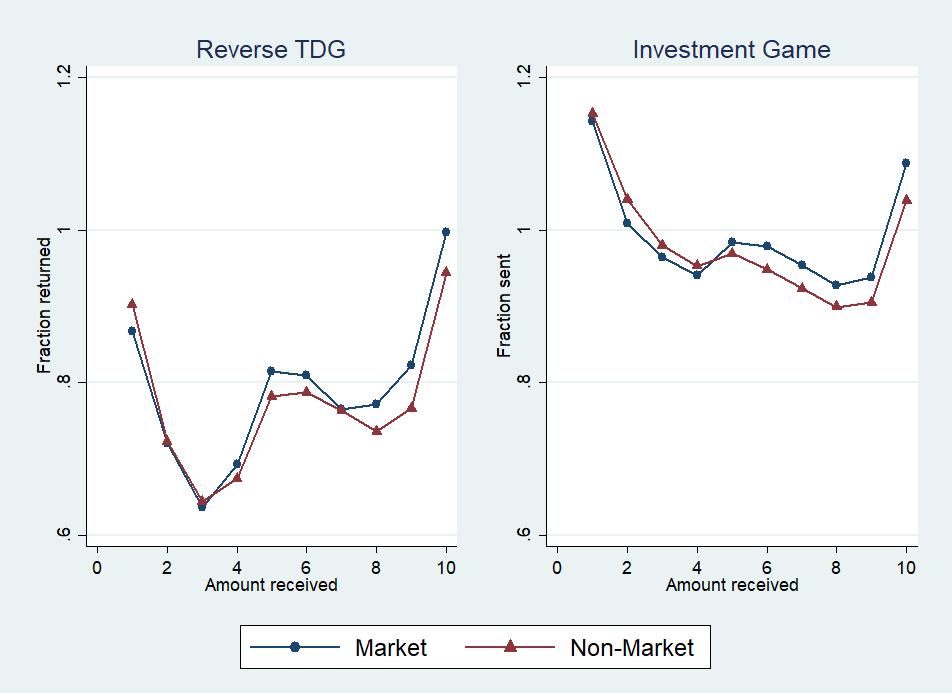
\includegraphics[width=0.8\linewidth]{C:/Users/Koen/Dropbox/PhD/Papers/CameroonTrust/Figures/Trustworthiness.png}
  \caption{Amounts sent in the rTGD and returned in the Investment Game}
  \label{fig:tw}
\end{figure}

It's immediately clear from figure \ref{fig:tw}  that levels are higher in the Investment Game. The fraction here varies around one, which corresponds to exactly returning the number of tokens received from the first mover. In comparing the market group with the non-market group, there are two quantities of interest: the mean fraction returned/sent over all rounds, and the slope of the line (as would be obtained by a simple regression of the the fraction on the round index). For the investment game, the mean fraction can be seen as an indicator for trustworthiness. A higher fraction means more of the amount received is returned to the first mover. The slope can be seen as an indicator for reciprocity. A respondent with a steeper slope, rewards higher amounts received more than low amounts. The results of the analysis of these two indicators is presented in Table \ref{tab:results_tw}. I include the values for the mean and slope of the rTDG as controls.

While, on average, participants in market communities are no more trustworthy than their counterparts in non-market communities, they are more reciprocal: they increase the fraction returned by a higher fraction when the amount received is increased. However, this effect is small: if the amount received is increased by 1 token, participants in market communities return 0.007 tokens more than non-market participants.


\begin{table}[htb]
	\small
	\caption{Results: trustworthiness}
	\label{tab:results_tw}
	\begin{center}
	{
\def\sym#1{\ifmmode^{#1}\else\(^{#1}\)\fi}
\begin{tabular}{l*{4}{c}}
\hline\hline
                    &\multicolumn{1}{c}{(1)}         &\multicolumn{1}{c}{(2)}         &\multicolumn{1}{c}{(3)}         &\multicolumn{1}{c}{(4)}         \\
                    &        Mean         &        Mean         &       Slope         &       Slope         \\
\hline
Market              &    0.000788         &     0.00477         &     0.00545         &     0.00614\sym{*}  \\
                    &    (0.0228)         &    (0.0432)         &   (0.00364)         &   (0.00364)         \\
[1em]
rTDG (mean)         &       0.688\sym{***}&       0.691\sym{***}&                     &                     \\
                    &    (0.0225)         &    (0.0318)         &                     &                     \\
[1em]
rTDG (mean) x Market&                     &    -0.00503         &                     &                     \\
                    &                     &    (0.0446)         &                     &                     \\
[1em]
rTGD (slope)        &                     &                     &       0.319\sym{***}&       0.358\sym{***}\\
                    &                     &                     &    (0.0215)         &    (0.0299)         \\
[1em]
rTDG (slope) x Market&                     &                     &                     &     -0.0714\sym{*}  \\
                    &                     &                     &                     &    (0.0424)         \\
[1em]
Constant            &       0.461\sym{***}&       0.458\sym{***}&     0.00232         &     0.00290         \\
                    &    (0.0729)         &    (0.0755)         &   (0.00708)         &   (0.00697)         \\
[1em]
Add. Controls       &         Yes         &         Yes         &         Yes         &         Yes         \\
\hline
N                   &        2185         &        2185         &        2185         &        2185         \\
Adj. R-Square       &        0.35         &        0.35         &        0.13         &        0.13         \\
\hline\hline
\end{tabular}
}

	\end{center}
\end{table}


%%%%%%%%%%%%%%%%%%%%%%%%%%%%%%%%
\section{Conclusion}
%%%%%%%%%%%%%%%%%%%%%%%%%%%%%%%%
This paper examined the role of market exposure in shaping the determinants of sending behaviour among participants of a trust game in Northern Cameroon. We consider three determinants: social preferences, risk preferences, and expectations. 

Our two main results are as follows: (i) in our sample, altruism explains more of the sending behaviour in the investment game than expectations; and (ii) expectations only drive trusting behaviour in the investment game in communities with markets, not in communities without markets.  

One possible explanation for increased cooperative behaviour in market societies is evolutionary: trusting behaviour in market communities is rewarded more than in non-market communities, which would lead to increased cooperation  over time (see e.g. \citep{Tabellini2008}). However, we find no evidence of such a process. We find that neither levels of expectations or altruism do not differ between market communities and non-market communities. Another explanation in line with literature on the on the link between rational behaviour and markets \citep[e.g.][]{List2008,Cecchi2013} is thus more likely. Due to more interactions with strangers, and more interactions with a market framing, people learn to respond to expectations more rationally.

These findings highlight the need to include ``non-standard'' populations matters for understanding human behaviour. In this case, sending behaviour in the trust game cannot simply be used as a proxy for trust, since the degree to which it correlates with expectations is different for different communities.


%bibliography, this is needed for bibtex
\clearpage 
\bibliographystyle{chicago}
%path to .bib file (e.g. automatically exported by mendeley) DO NOT include the file extension!
\bibliography{C:/Users/Koen/Dropbox/Literatuur/Mendeley/Bibtex/CameroonTrust}


\clearpage
\section{Appendix}
\setcounter{table}{0}
\renewcommand{\thetable}{A\arabic{table}}

\begin{table}[hp] \centering
\newcolumntype{C}{>{\centering\arraybackslash}X}

\caption{Covariate balance, before matching}
\label{tab:balance_noweight}
{\footnotesize
\begin{tabularx}{\linewidth}{lCCCCCCC}

\toprule
&{(1)}&{(2)}&{(3)}&{(4)}&{(5)}&{(6)}&{(7)} \tabularnewline
&\multicolumn{2}{c}{All}&\multicolumn{2}{c}{Treatment}&\multicolumn{2}{c}{Control}&{(4)-(6)}\tabularnewline \midrule
{}&{N}&{Mean}&{N}&{Mean}&{N}&{Mean}&{ } \tabularnewline
\midrule \addlinespace[\belowrulesep]
Married&3195&0.78&1808&0.76&1387&0.80&--0.03* \tabularnewline
&&(0.42)&&(0.42)&&(0.40)& \tabularnewline
Village Size&3278&173.42&1851&236.21&1427&91.97&144.24*** \tabularnewline
&&(139.72)&&(152.53)&&(54.04)& \tabularnewline
HH Size&3164&7.32&1784&7.42&1380&7.19&0.23 \tabularnewline
&&(4.83)&&(4.98)&&(4.62)& \tabularnewline
Muslim&3164&0.81&1784&0.83&1380&0.79&0.04 \tabularnewline
&&(0.39)&&(0.37)&&(0.41)& \tabularnewline
Number of wives&2272&1.57&1262&1.63&1010&1.49&0.14*** \tabularnewline
&&(0.87)&&(0.92)&&(0.79)& \tabularnewline
Village leader&3195&0.06&1808&0.06&1387&0.07&--0.01* \tabularnewline
&&(0.24)&&(0.23)&&(0.25)& \tabularnewline
Head educated&3164&0.40&1784&0.42&1380&0.37&0.05 \tabularnewline
&&(0.49)&&(0.49)&&(0.48)& \tabularnewline
Age HH head&3164&44.54&1784&44.59&1380&44.48&0.11 \tabularnewline
&&(16.09)&&(15.92)&&(16.31)& \tabularnewline
Improved roof&3157&0.56&1779&0.64&1378&0.46&0.18*** \tabularnewline
&&(0.50)&&(0.48)&&(0.50)& \tabularnewline
High wellbeing relative to village&2633&0.18&1483&0.18&1150&0.17&0.01 \tabularnewline
&&(0.38)&&(0.39)&&(0.38)& \tabularnewline
\bottomrule \addlinespace[\belowrulesep]

\end{tabularx}
\begin{flushleft}
\footnotesize Standard Deviations in parantheses; *p $<$ 0.1,**p $<$ 0.05,***p $<$ 0.01
\end{flushleft}
}
\end{table}

\begin{table}[hp] \centering
\newcolumntype{C}{>{\centering\arraybackslash}X}

\caption{Covariate balance, after matching}
\label{tab:balance_weight}
{\footnotesize
\begin{tabularx}{\textwidth}{lCCCCCCC}

\toprule
&{(1)}&{(2)}&{(3)}&{(4)}&{(5)}&{(6)}&{(7)} \tabularnewline
&\multicolumn{2}{c}{All}&\multicolumn{2}{c}{Treatment}&\multicolumn{2}{c}{Control}&{(4)-(6)}\tabularnewline
{}&{N}&{Mean}&{N}&{Mean}&{N}&{Mean}&{ } \tabularnewline
\midrule\addlinespace[1.5ex]
Married&3144&0.77&1783&0.76&1361&0.78&-0.02 \tabularnewline
&&(0.42)&&(0.43)&&(0.41)& \tabularnewline
Village Size&3220&174.15&1825&235.46&1395&93.95&141.51*** \tabularnewline
&&(139.26)&&(152.42)&&(55.04)& \tabularnewline
HH Size&3108&7.44&1758&7.43&1350&7.46&-0.03 \tabularnewline
&&(4.93)&&(4.97)&&(4.88)& \tabularnewline
Muslim&3108&0.83&1758&0.83&1350&0.83&0.00 \tabularnewline
&&(0.37)&&(0.37)&&(0.37)& \tabularnewline
Number of wives&2232&1.61&1241&1.63&991&1.58&0.06 \tabularnewline
&&(0.88)&&(0.91)&&(0.82)& \tabularnewline
Village leader&3144&0.05&1783&0.05&1361&0.05&-0.00 \tabularnewline
&&(0.23)&&(0.23)&&(0.23)& \tabularnewline
Head educated&3108&0.42&1758&0.42&1350&0.42&0.00 \tabularnewline
&&(0.49)&&(0.49)&&(0.49)& \tabularnewline
Age HH head&3108&44.78&1758&44.84&1350&44.69&0.16 \tabularnewline
&&(15.52)&&(15.47)&&(15.60)& \tabularnewline
Improved roof&3103&0.57&1754&0.64&1349&0.48&0.16*** \tabularnewline
&&(0.50)&&(0.48)&&(0.50)& \tabularnewline
High wellbeing relative to village&2589&0.18&1460&0.18&1129&0.18&0.01 \tabularnewline
&&(0.39)&&(0.39)&&(0.38)& \tabularnewline
\bottomrule \addlinespace[1.5ex]

\end{tabularx}
\begin{flushleft}
\footnotesize Standard Deviations in parantheses; *p $<$ 0.1,**p $<$ 0.05,***p $<$ 0.01
\end{flushleft}
}
\end{table}



